\documentclass{beamer}

% PACKAGES
% ----------------------------------------------------------------------------
\usetheme{Berlin}
\usepackage{graphicx}
\usepackage[latin1]{inputenc}
\usepackage[english]{babel}
\usepackage{hyperref}

% SETTINGS
% ----------------------------------------------------------------------------
\makeatletter
\let\beamer@writeslidentry@miniframeson=\beamer@writeslidentry
\def\beamer@writeslidentry@miniframesoff{%
  \expandafter\beamer@ifempty\expandafter{\beamer@framestartpage}{}% does not happen normally
  {%else
    % removed \addtocontents commands
    \clearpage\beamer@notesactions%
  }
}
\newcommand*{\miniframeson}{\let\beamer@writeslidentry=\beamer@writeslidentry@miniframeson}
\newcommand*{\miniframesoff}{\let\beamer@writeslidentry=\beamer@writeslidentry@miniframesoff}
\makeatother
\beamertemplatenavigationsymbolsempty
\makeatletter
\beamer@theme@subsectionfalse%
\makeatother
\setbeamertemplate{footline}
{%
\begin{beamercolorbox}[wd=1.0\textwidth,ht=2.6ex,dp=1ex,leftskip=.5em,rightskip=.5em]{author in head/foot}%
\usebeamerfont{author in head/foot}%
\insertshortauthor\hfill\insertshortinstitute%
%\insertframenumber{} von \inserttotalframenumber\hfill\insertshortauthor%
\end{beamercolorbox}%
%\hspace*{-4.0ex}\hspace*{0.3\textwidth}%
\begin{beamercolorbox}[wd=1.0\textwidth,ht=2.6ex,dp=1ex,left,leftskip=.5em,rightskip=.5em]{title in head/foot}%
\usebeamerfont{title in head/foot}%
\insertshorttitle\hfill\insertframenumber{} / \inserttotalframenumber%
\end{beamercolorbox}%
}
\setbeamerfont{footnote}{size=\tiny}

% CONFIGURE TITLEPAGE
% ----------------------------------------------------------------------------
\title{Explicit Sentiment Analysis with Language Patterns about Uncertainty}
\subtitle{Project Presentation}
\author{Jan Albrecht, Paul Brassel, Pascal Singer}
\institute[]{Group: \glqq We're not quite sure what we're doing\grqq \\ \vspace{0.3cm} Universit�t Leipzig \\
Big Data and Language Technologies Seminar}
\date{04th July 2022}
\titlegraphic{\vspace{0.2cm}\hspace{8cm}
\includegraphics[scale=0.25]{logo.png}}

% DOCUMENT
% ----------------------------------------------------------------------------
\begin{document}

\miniframesoff

\begin{frame}
	\titlepage
\end{frame}

\begin{frame}{Goals}
	\begin{itemize}
		\item[1.] Extract a dataset about semantic uncertainty from the web archive data.
		\begin{itemize}
			\setlength\itemsep{5pt}
			\item use specific language patterns about uncertainty
			\item classify samples into positive/negative sentiments
			\item compare dataset to sentiment140\footnotemark
		\end{itemize}
		\item[2.] Train a sentiment classifier based on DistilBERT on our dataset using transfer learning.
		\begin{itemize}
			\setlength\itemsep{5pt}
			\item classifier is finetuned on SST-2\footnotemark
			\item benchmark our classifier on sentiment140
		\end{itemize}
	\end{itemize}
	\footnotetext[1]{\url{https://huggingface.co/datasets/sentiment140}}
	\footnotetext[2]{\url{https://huggingface.co/distilbert-base-uncased-finetuned-sst-2-english}}
\end{frame}

\begin{frame}{Language Patterns}
	\begin{figure}[htb]
		\centering
		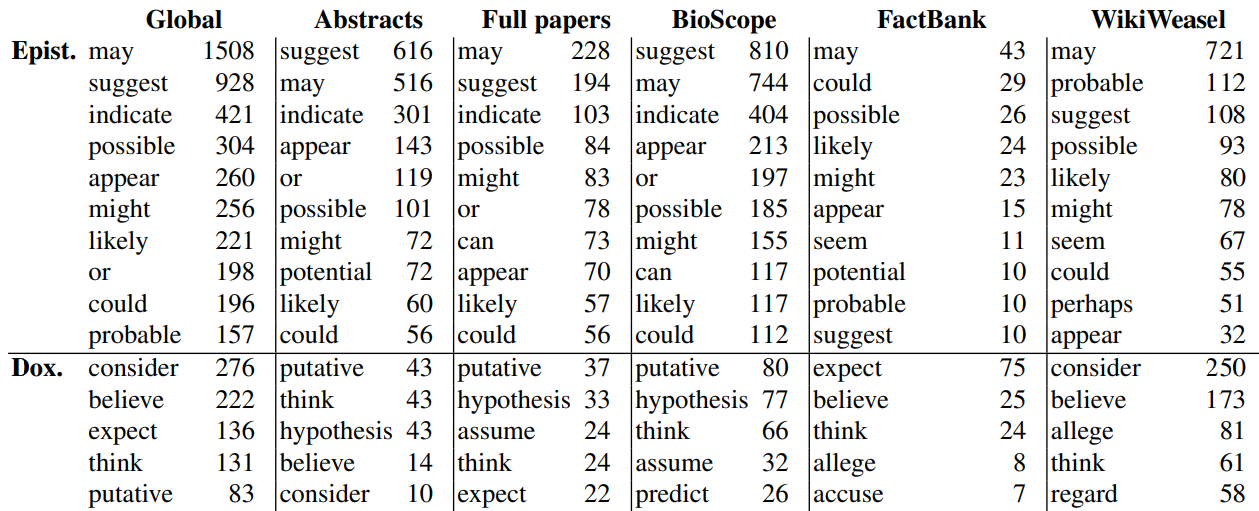
\includegraphics[scale=0.3]{language_patterns_cutting.png}
		\caption{The most frequent cues in the English corpora.\footnotemark}
	\end{figure}
	\vspace{-0.3cm}
	\begin{itemize}
		\item[$\rightarrow$] Does these frequency distribution correspond to our dataset?
	\end{itemize}
	\footnotetext[3]{\url{http://doktori.bibl.u-szeged.hu/id/eprint/2291/1/Vincze_Veronika_tezis.pdf}, p. 43}
\end{frame}

\begin{frame}{Dataset}
\end{frame}

\begin{frame}{Model}
\end{frame}

\end{document}